%  article.tex (Version 3.3, released 19 January 2008)
%  Article to demonstrate format for SPIE Proceedings
%  Special instructions are included in this file after the
%  symbol %>>>>
%  Numerous commands are added out, but included to show how
%  to effect various options, e.g., to print page numbers, etc.
%  This LaTeX source file is composed for LaTeX2e.

%  The following commands have been added in the SPIE class
%  file (spie.cls) and will not be understood in other classes:
%  \supit{}, \authorinfo{}, \skiplinehalf, \keywords{}
%  The bibliography style file is called spiebib.bst,
%  which replaces the standard style unstr.bst.

%\documentclass[a4paper]{spie}
\documentclass[]{spie}  %>>> use for US letter paper
%%\documentclass[a4paper]{spie}  %>>> use this instead for A4 paper
%%\documentclass[nocompress]{spie}  %>>> to avoid compression of citations
%% \addtolength{\voffset}{9mm}   %>>> moves text field down
%% \renewcommand{\baselinestretch}{1.65}   %>>> 1.65 for double spacing, 1.25 for 1.5 spacing
%  The following command loads a graphics package to include images
%  in the document. It may be necessary to specify a DVI driver option,
%  e.g., [dvips], but that may be inappropriate for some LaTeX
%  installations.
\usepackage[]{graphicx}
\usepackage{color}
\usepackage{cancel}
\usepackage{amsmath}
\usepackage{mathtools}
\usepackage{verbatim}
\usepackage{titlesec}
\definecolor{linkcolor}{cmyk}{1, 0.65, 0, 0.3}			% PANTONE 288 CVU
\definecolor{citecolor}{cmyk}{0.79, 0, 0.87, 0.56}		% PANTONE 357 CVU
%\definecolor{citecolor}{cmyk}{1, 0, 0.47, 0.3}			% PANTONE 328
\def\red{\textcolor{red}}
\def\blue{\textcolor{blue}}
\usepackage[
	colorlinks,
	linkcolor=linkcolor,
	urlcolor=linkcolor,
	citecolor=linkcolor,
	pdftex,
	pdfstartview=FitH,
]{hyperref}

\titleformat{\section}{\normalfont\fontsize{11.5pt}{1em}\bfseries}{SUPPLEMENTARY NOTE \thesection: }{0em}{}
\titleformat{\subsection}{\normalfont\fontsize{11pt}{0.75em}\bfseries}{SUPPLEMENTARY NOTE \thesubsection: }{0em}{}
\titleformat{\subsubsection}{\normalfont\fontsize{11pt}{0.75em}\bfseries}{SUPPLEMENTARY NOTE \thesubsubsection: }{0em}{}

% jump to the top of a figure, not the caption
\usepackage[all]{hypcap}

% so that footnotes in tables work
\usepackage{footnote}

% so that we can omit the 'Table 1:' for the overview
\usepackage{caption}

% should be called Supplementary Figure
\renewcommand{\figurename}{Supplementary Figure}

% for the source code
\usepackage{listings}

\usepackage{helvet}
\renewcommand{\rmdefault}{\sfdefault}
\renewcommand{\baselinestretch}{1.05}

%\usepackage{sectsty}Bayesian-based single-view and multi-view deconvolution
%\allsectionsfont{\sffamily}

\captionsetup[table]{labelformat=empty}

\newcommand\smallurl[1]{{\small{\url{#1}}}}
\newcommand\tablespace{\vspace{2.5mm}}
\newcommand\fig{supplementary figure }
\newcommand\Fig{Supplementary figure }


\title{BigStitcher: Efficient alignment of large multi-tile and multi-view image datasets}

%>>>> The author is responsible for formatting the
%  author list and their institutions.  Use  \skiplinehalf
%  to separate author list from addresses and between each address.
%  The correspondence between each author and his/her address
%  can be indicated with a superscript in italics,
%  which is easily obtained with \supit{}.

\author{David H{\"o}rl, Fabio Rojas Rusak, Stephan Preibisch
%\skiplinehalf
%\small{
%\supit{1}Max Planck Institute of Molecular Cell Biology and Genetics, Pfotenhauerstrasse 108, Dresden, Germany \\
%\supit{2}HHMI Janelia Farm Research Campus, 19700 Helix Drive, Ashburn, VA 20147, USA \\
%\supit{3}Albert Einstein College of Medicine, 1300 Morris Park Avenue, Bronx, NY 10461, USA
%}
}

%>>>> Further information about the authors, other than their
%  institution and addresses, should be included as a footnote,
%  which is facilitated by the \authorinfo{} command.

%\authorinfo{Further author information: (Send correspondence to A.A.A.)\\A.A.A.: E-mail: aaa@tbk2.edu, Telephone: 1 505 123 1234\\  B.B.A.: E-mail: bba@cmp.com, Telephone: +33 (0)1 98 76 54 32}
%%>>>> when using amstex, you need to use @@ instead of @


%%%%%%%%%%%%%%%%%%%%%%%%%%%%%%%%%%%%%%%%%%%%%%%%%%%%%%%%%%%%%
%>>>> uncomment following for page numbers
\pagestyle{plain}
%>>>> uncomment following to start page numbering at 301
%\setcounter{page}{1}

\begin{document}

\maketitle

%\pagestyle{headings}
\setcounter{page}{1}
\pagenumbering{roman}
\pagenumbering{arabic}


\hspace{20mm}

\begin{table}[h!]
\center
{
\fontsize{12pt}{11pt}\selectfont
\center
\begin{tabular}{lp{11cm}}
\textbf{\textcolor{red}{Supplementary File}} & \textbf{\textcolor{red}{Title}}\\ \\
\hline
\\
\textbf{Supplementary Figure \ref{fig:ds-stats-01}} & Downsampling error statistics \tablespace \\
\textbf{Supplementary Figure \ref{fig:ds-stats-02}} & Per-axis downsampling error statistics \tablespace \\
\textbf{Supplementary Figure \ref{fig:downsampling}} &  Downsampling with different SNR \tablespace \\
\textbf{Supplementary Figure \ref{fig:stitching}} & Example stitching \tablespace \\
\textbf{Supplementary Note \ref{sec:sup-methods}} & Supplementary methods \tablespace \\
\textbf{Supplementary Note \ref{sec:documentation}} & BigStitcher user guide \tablespace \\
\textbf{Supplementary Note \ref{sec:currentcode}} & Links to the current source codes \tablespace \\
\end{tabular}}
\caption{\emph{Note: Supplementary Videos 1--XXX are available for download on the journal homepage.}}
\end{table}

\pagebreak

\titleformat{\section}{\centering\normalfont\fontsize{11.5pt}{1em}\bfseries}{SUPPLEMENTARY NOTE \thesection: }{0em}{}
\section*{SUPPLEMENTARY FIGURES}
\titleformat{\section}{\normalfont\fontsize{11.5pt}{1em}\bfseries}{SUPPLEMENTARY NOTE \thesection: }{0em}{}

\hspace{20mm}

\subsection*{SUPPLEMENTARY FIGURE 1: Downsampling error statistics}

\vspace{1mm}

\begin{figure*}[h!]
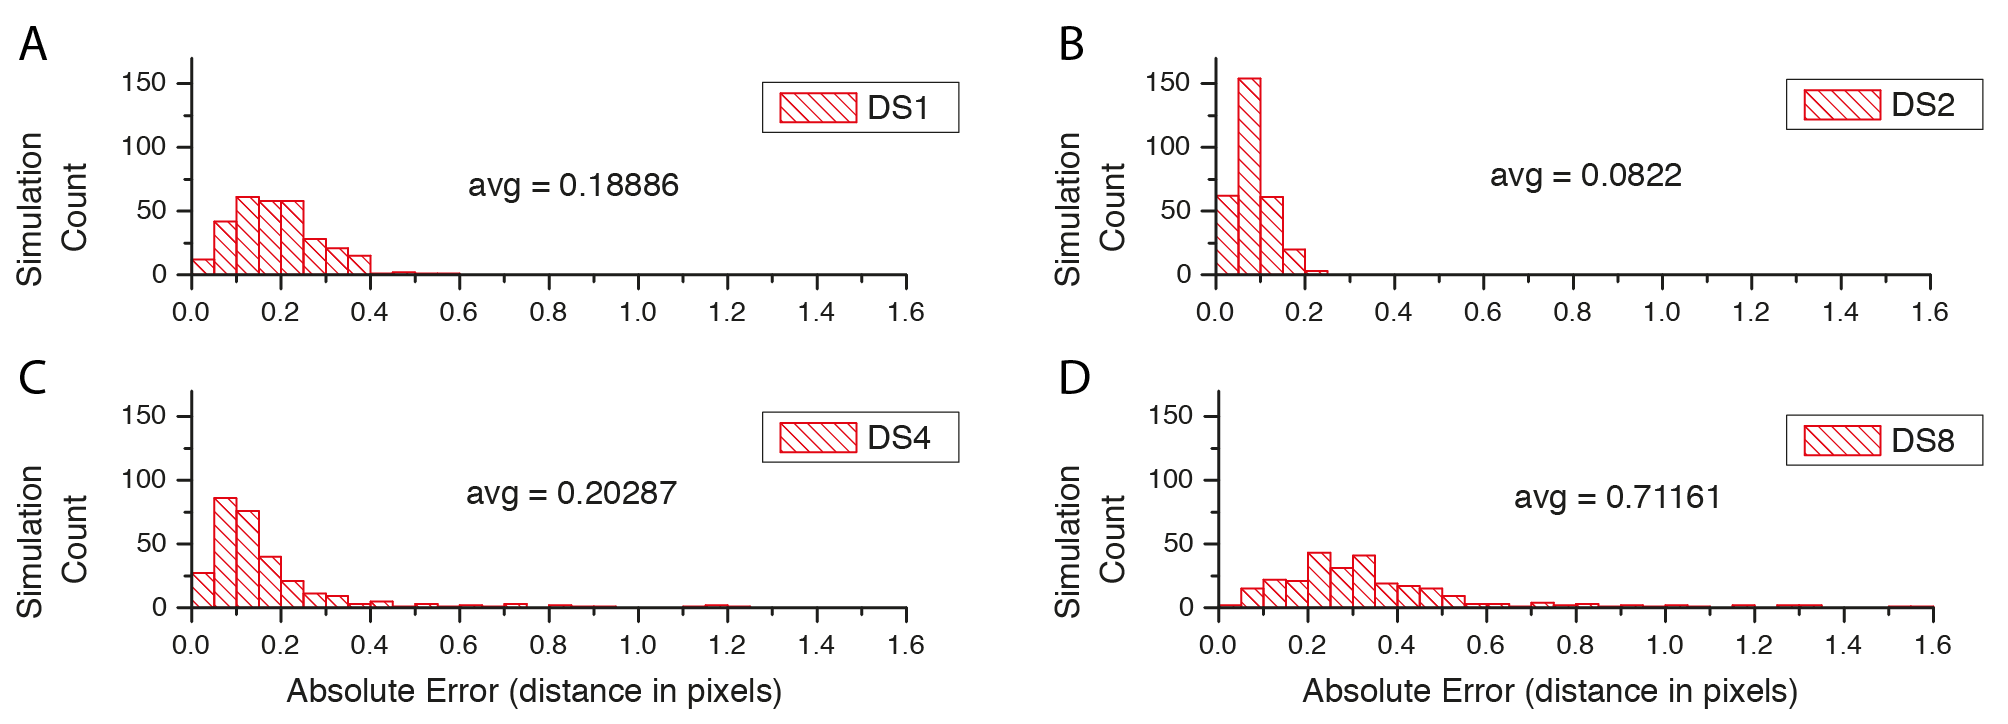
\includegraphics[width=\textwidth]{fig-downsampling-statistics-1.png}
\vspace{-2.0mm}
\caption{\hspace{-0.5mm} \emph{Illustration of conditional probabilities describing the dependencies of two views.} \mbox{(\textbf{a}) illustrates} the conditional independence of two observed distributions $\phi_1(x_1)$ and $\phi_2(x_2)$ if it is known that the event $\xi=\xi'$ on the underlying distribution $\psi(\xi)$ occured. Given $\xi=\xi'$, both distributions are conditionally independent, the probability where to expect an observation only depends on $\xi=\xi'$ and the respective individual point spread function $P(x_1|\xi)$ and $P(x_2|\xi)$, i.e. $P(x_1|\xi,x_2) = P(x_1|\xi)$ and $P(x_2|\xi,x_1) = P(x_2|\xi)$. \mbox{(\textbf{b}) illustrates} the relationship between an observed distribution $\phi_2(x_2)$ and $\phi_1(x_1)$ if the event $x_1=x_1'$ occured. Solely the 'inverse' point spread function $Q(\xi|x_1)$ defines the probability for any event $\xi=\xi'$ to have caused the observation $x_1=x_1'$. The point spread function $P(x_2|\xi)$ consecutively defines the probability where to expect a corresponding observation $x_2=x_2'$ given the probability distribution $\psi(\xi)$.
}
\label{fig:ds-stats-01}
\end{figure*}

\pagebreak

\vspace{10mm}

\subsection*{SUPPLEMENTARY FIGURE 2: The principle of 'virtual' views and sequential updating}

\vspace{1mm}

\begin{figure*}[h!]
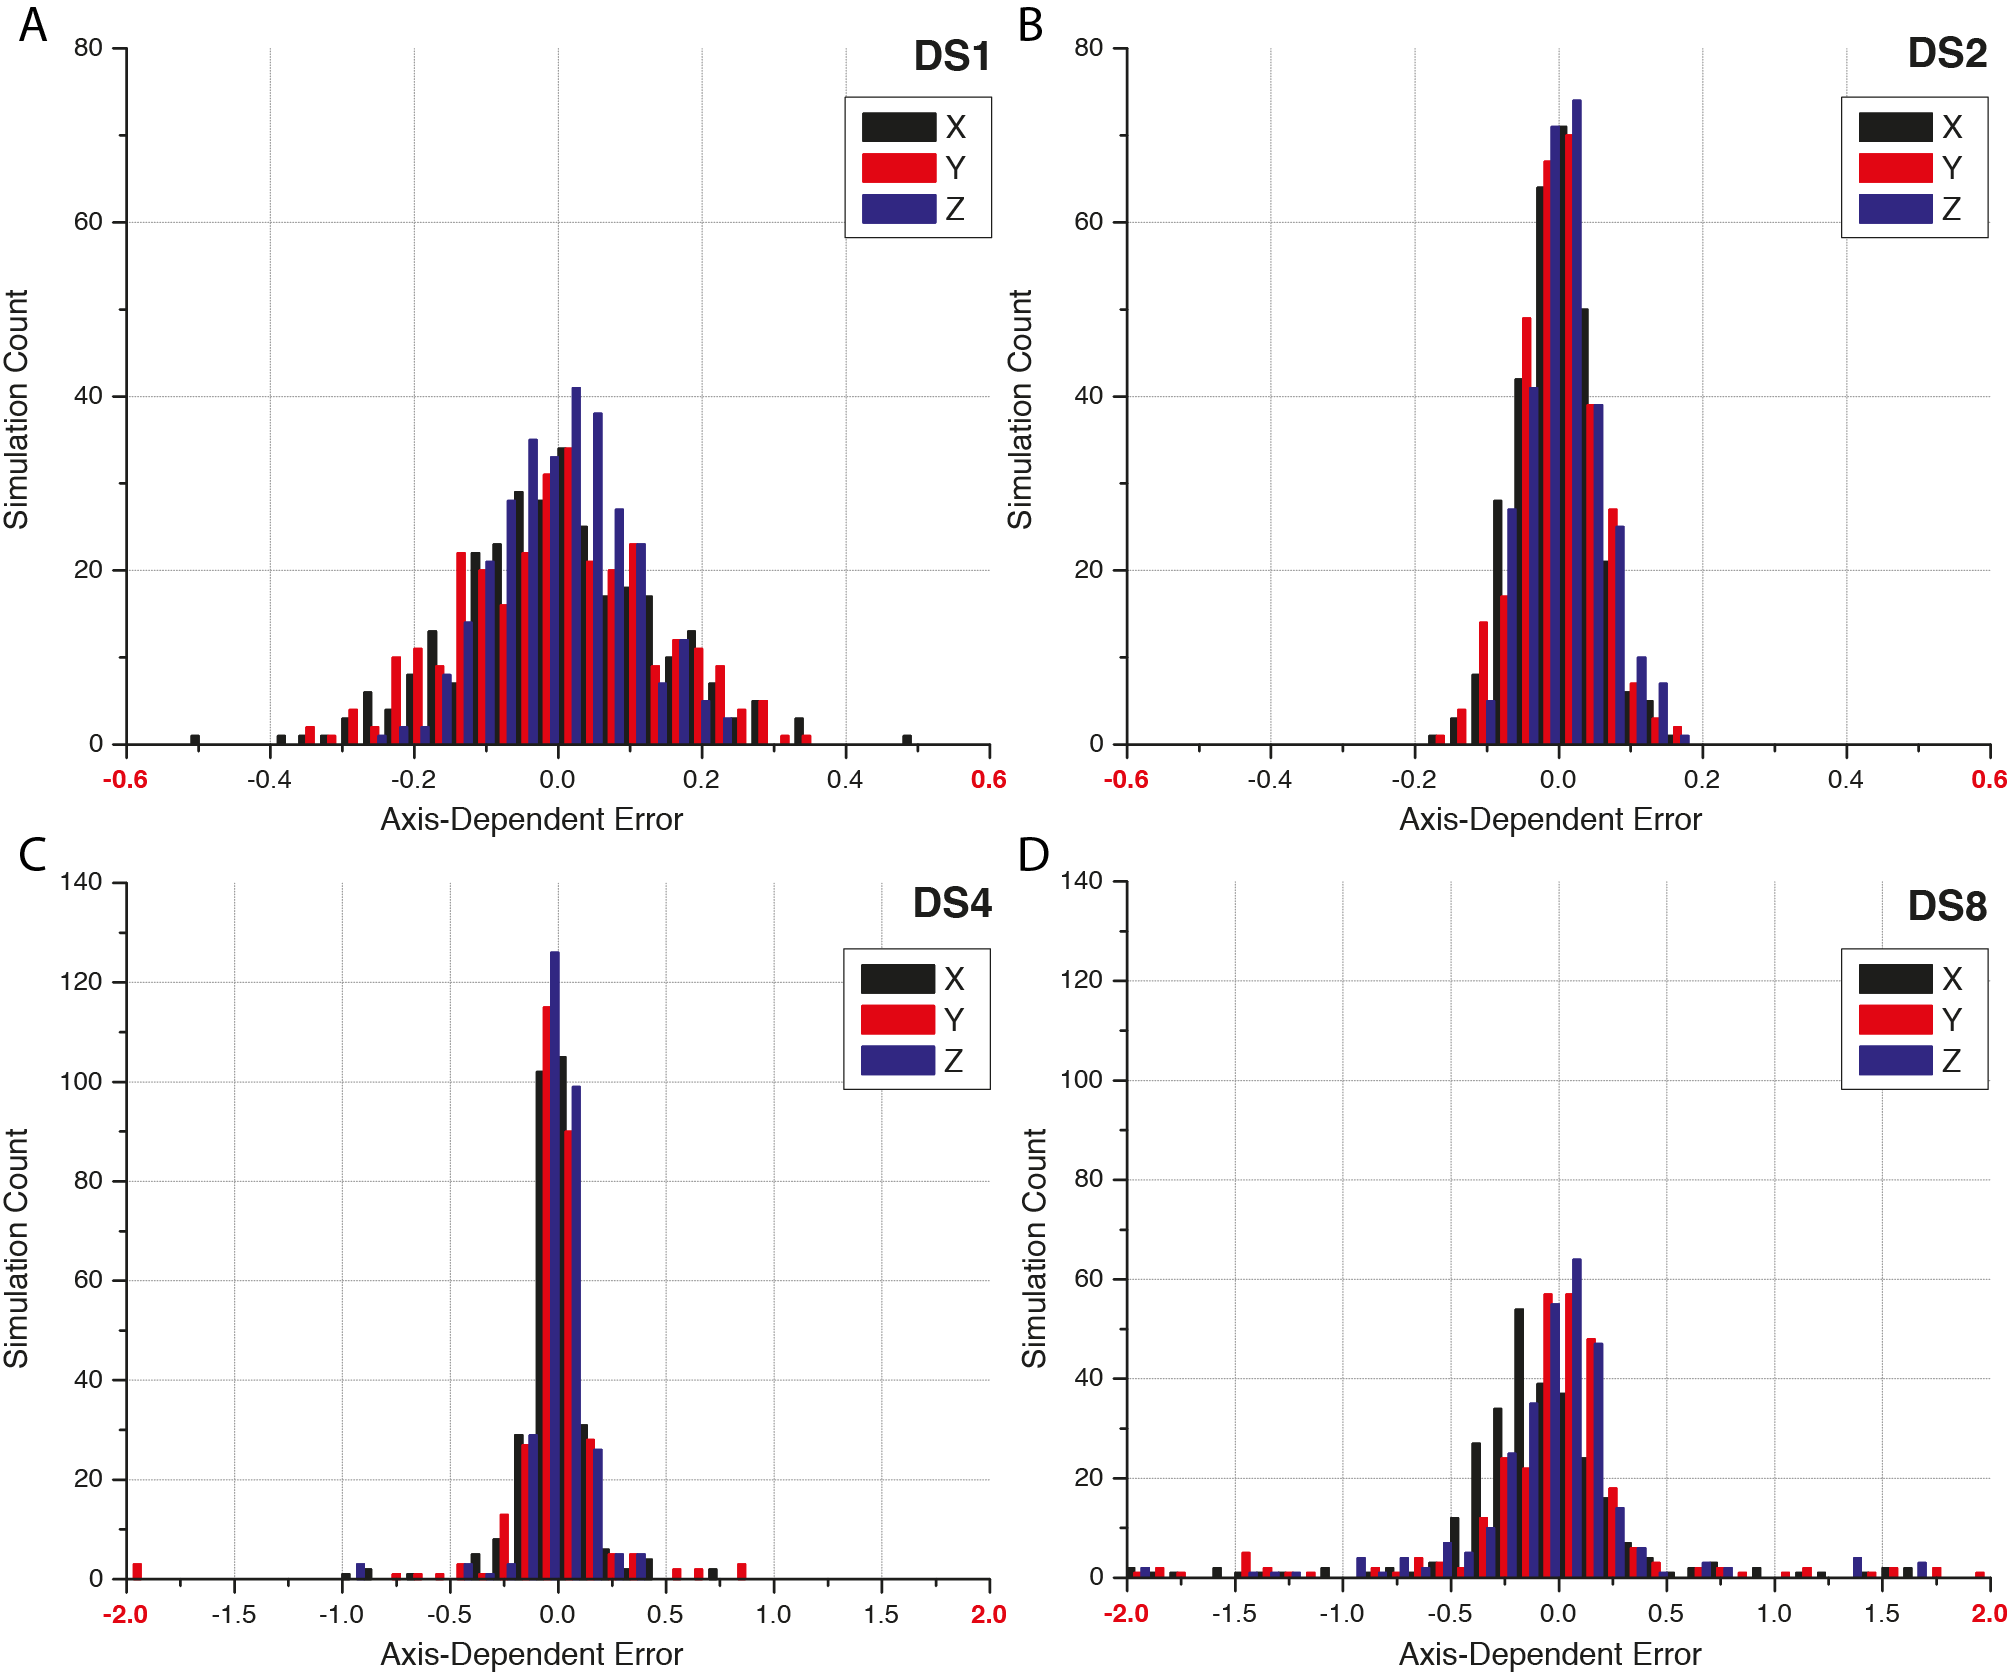
\includegraphics[width=\textwidth]{fig-downsampling-statistics-2.png}
\vspace{-2.0mm}
\caption{\hspace{-0.5mm}\emph{The principle of 'virtual' views and sequential updating.} (\textbf{a}) The ‘classical’ multi-view deconvolution\cite{Shepp1982, KrzicPhD, Temerinac2012, Bonetti2009} where an update step is computed individually for each view and subsequently combined into one update of the deconvolved image. (\textbf{b}) Our new derivation considering conditional probabilities between views. Each individual update step takes into account all other views using ‘virtual views’ and additionally updates the deconvolved image individually, i.e. updates are performed sequentially\cite{Hudson1994} and not combined.
}\label{fig:ds-stats-02}
\end{figure*}

\pagebreak

\subsection*{SUPPLEMENTARY FIGURE 3: Illustration of assumption required for incorporating 'virtual' views without additional computational effort}

\vspace{1mm}

\begin{figure*}[h!]
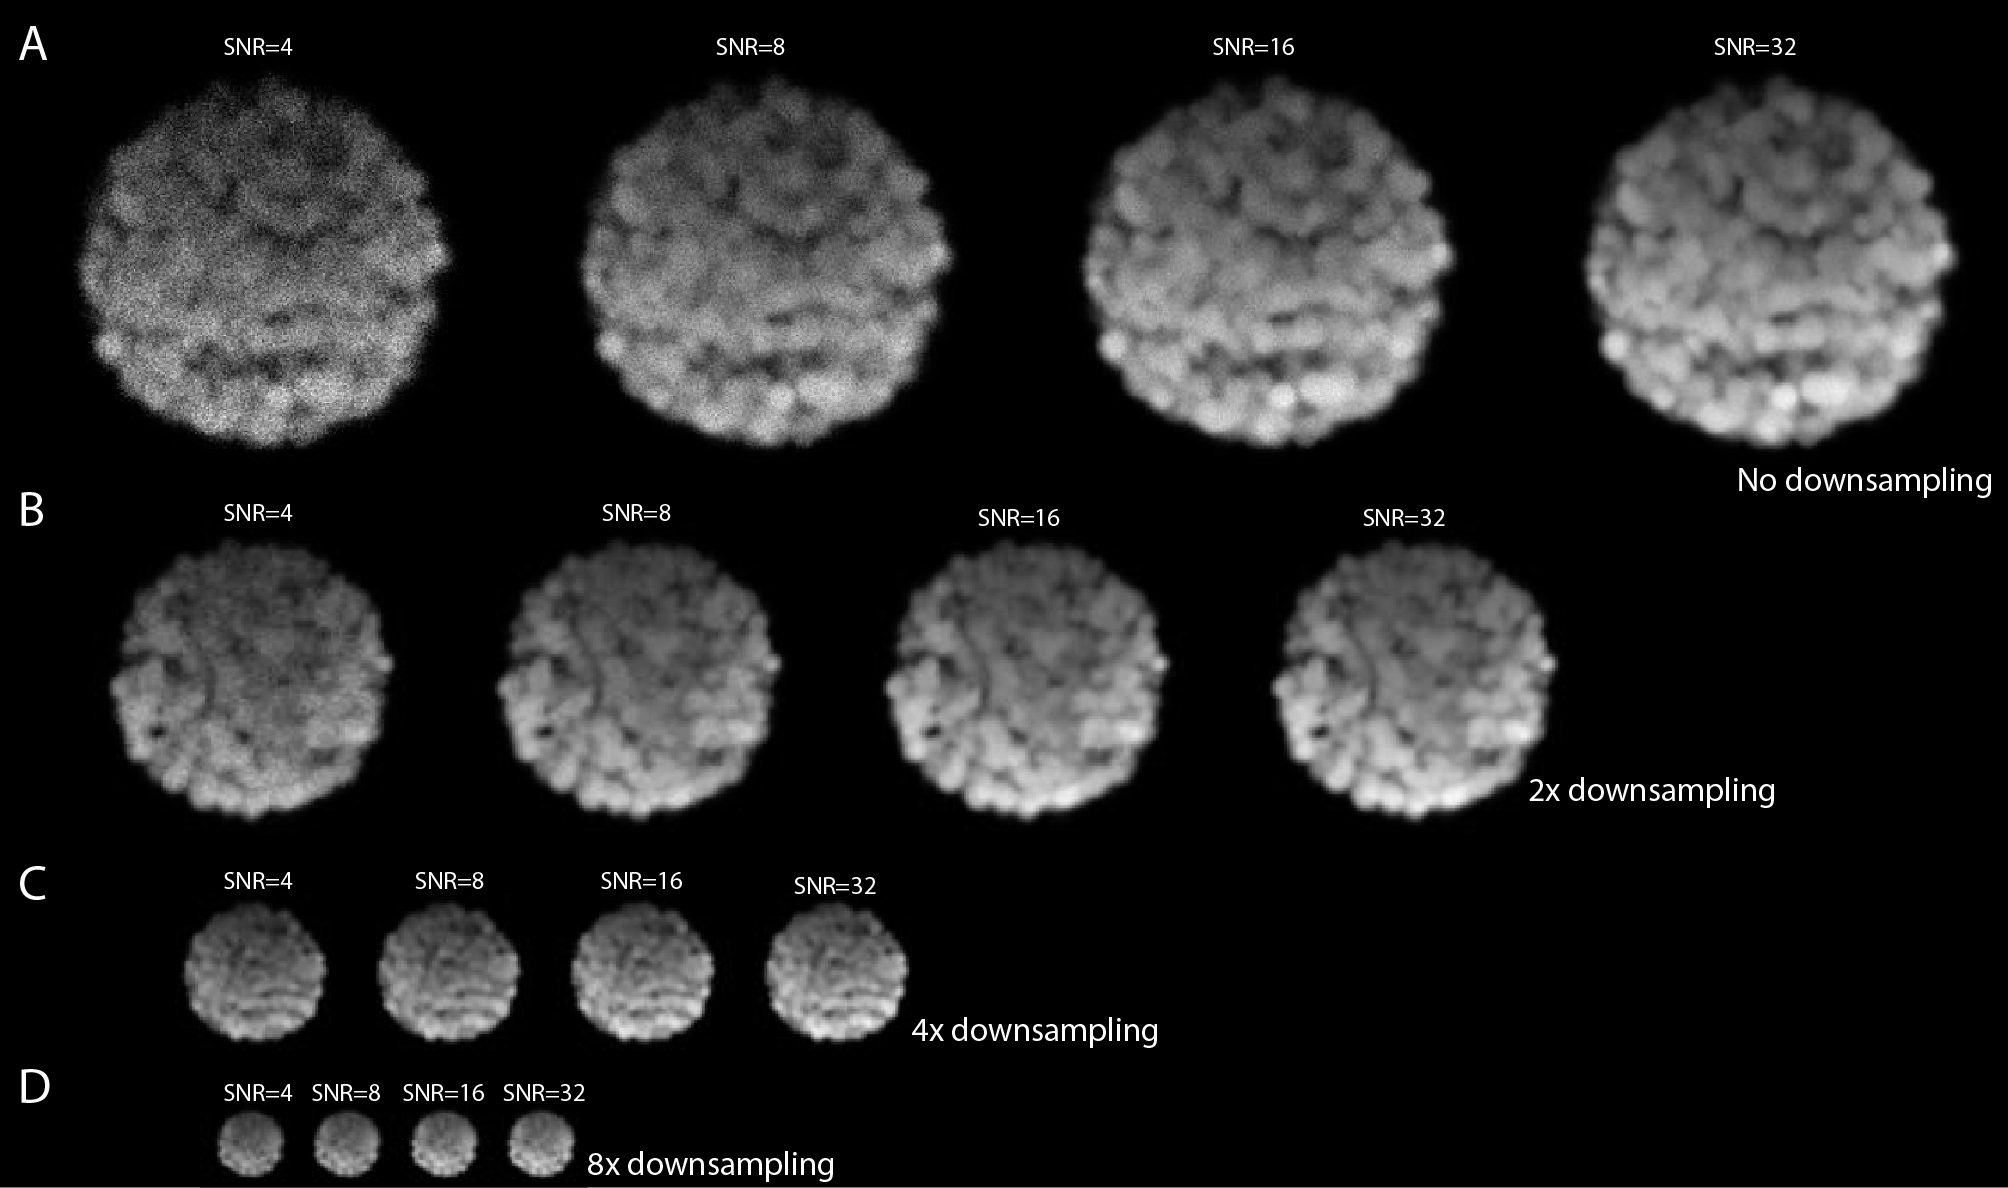
\includegraphics[width=\textwidth]{fig-downsampling.png}
\vspace{-2.0mm}
\caption{\hspace{-0.5mm}\emph{Illustration of assumption in equation \ref{eq:eq210}.} (\textbf{a}) shows the difference in the result when computing $( f \ast g ) \cdot ( f \ast h )$ in red and the approximation $f \ast ( g \cdot h )$ in black for a random one-dimensional input sequence ($f$) and two kernels with $\sigma$=3 ($g$) and $\sigma$=2 ($h$) after normalization. (\textbf{b}) shows the difference when using the two-dimensional image from \fig \ref{fig:viewsimages}a as input ($f$) and the first two point spread functions from \fig \ref{fig:viewsimages}e as kernels ($g,h$). The upper panel pictures the approximation, the lower panel the correct computation. Note that for (\textbf{a,b}) the approximation is slightly less blurred. Note that the beads are also visible in the lower panel when adjusting the brightness/contrast.
}\label{fig:downsampling}
\end{figure*}

\pagebreak

\subsection*{SUPPLEMENTARY FIGURE 4: Performance comparison of the multi-view deconvolution methods and dependence on the PSF}

\vspace{1mm}

\begin{figure*}[h!]
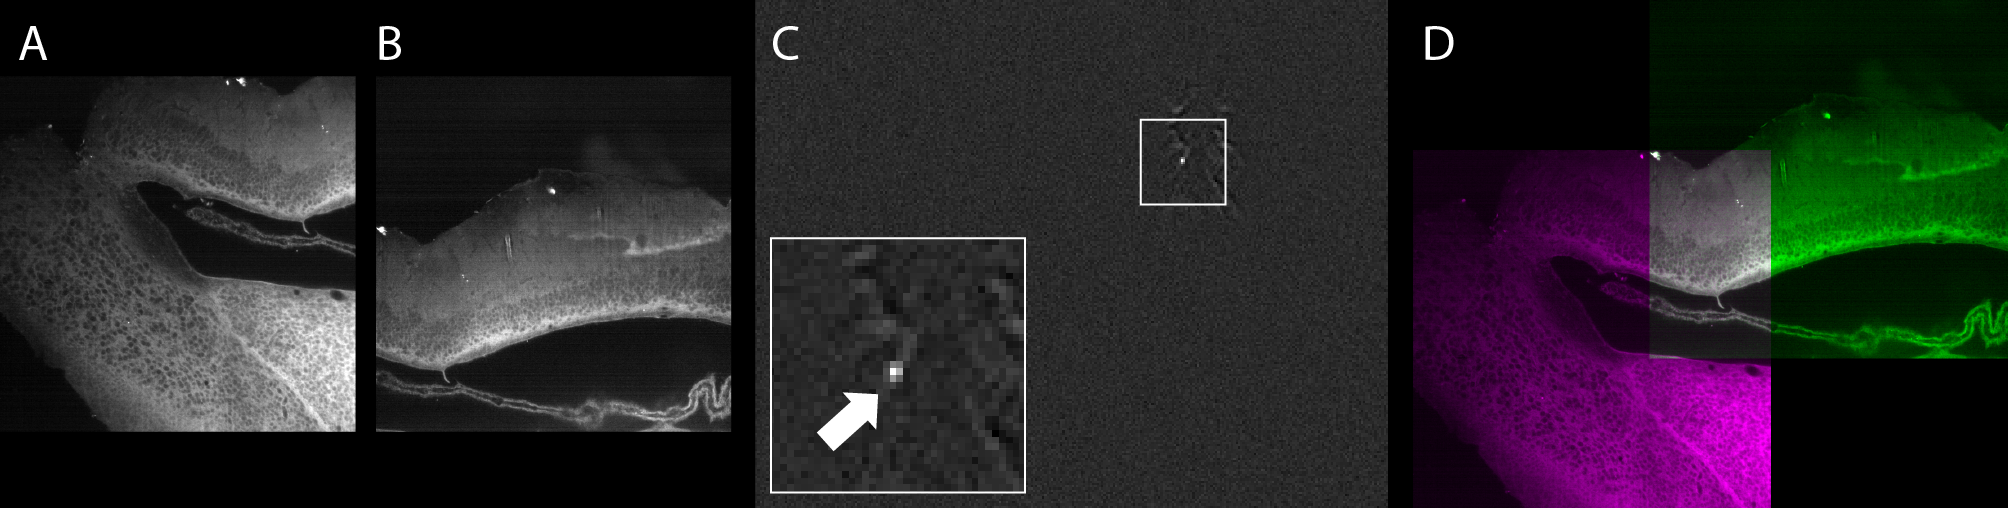
\includegraphics[width=\textwidth]{fig-stitching.png}
\vspace{-2.0mm}
\caption{\hspace{-0.5mm}\emph{Performance comparison and dependence on the PSF} (\textbf{a}) The convergence time of the different algorithms until they reach the same average difference to the ground truth image shown in \fig \ref{fig:viewsimages}e. (\textbf{b}) The number of iterations required until all algorithms reach the same average difference to the ground truth image. One 'iteration' comprises all computional steps until each view contributed once to update the underlying distribution. Note that our Bayesian-based derivation and the Maximization-Likelihood Expectation-Maximization\cite{Shepp1982} method perform almost identical (\textbf{c}) The total number of updates of the underlying distribution until the same average difference is reached. (\textbf{d}) The number of iterations required until the same difference to the ground truth is achieved using 4 views. The number of iterations is plotted relative to the angular difference between the input PSFs. An angular difference of 0 degrees refers to 4 identical PSFs and therefore 4 identical input images, an example of an angular difference of 45 degrees is shown in \fig \ref{fig:viewsimages}e. Plots are shown for different types of PSFs. (\textbf{a-d}) y-axis has logarithmic scale, all computations were performed on a dual-core Intel Core i7 with 2.7Ghz.
}\label{fig:stitching}
\end{figure*}

\pagebreak



\titleformat{\section}{\centering\normalfont\fontsize{11.5pt}{1em}\bfseries}{SUPPLEMENTARY NOTE \thesection: }{0em}{}
\section*{SUPPLEMENTARY TABLES}
\titleformat{\section}{\normalfont\fontsize{11.5pt}{1em}\bfseries}{SUPPLEMENTARY NOTE \thesection: }{0em}{}

%========old table========
\begin{comment}

\hspace{20mm}

\subsection*{SUPPLEMENTARY TABLE 1: Summary of datasets used in this publication}

\hspace{20mm}

\setcounter{table}{0}
\newcounter{savecntr1}% Save footnote counter
\newcounter{restorecntr1}% Restore footnote counter
\newcounter{savecntr2}% Save footnote counter
\newcounter{restorecntr2}% Restore footnote counter

\begin{savenotes}
\begin{table}[h!]
\center
{
\fontsize{9pt}{10pt}\selectfont
\center
\begin{tabular}{p{5.5cm}p{3.0cm}p{3.6cm}p{3.5cm}}
\textbf{Dataset} & \textbf{Size, Lightsheet} & \textbf{Computation Time,} & \textbf{Machine}\\
 & \textbf{Thickness, SNR\footnote{The SNR is estimated by M.S., E.M., and P.T. were additionally supported by the Bundesministerium für Bildung und Forschung grant 031A099.computing the average intensity of the signal, divided by the standard deviation of the signal in areas with homogenous sample intensity}}  &\textbf{Iterations, Method} &  \\
\\
\hline
\\
\emph{Drosophila} embryo expressing His-YFP in all cells  acquired with Zeiss SPIM prototype using a 20x/0.5 detection objective (\textbf{Fig. 2c-e}, \textbf{Supp. Fig. \ref{fig:resolution}})\setcounter{savecntr1}{\value{footnote}}\footnote{This SPIM acquisition was already used in Preibisch (2010)\cite{Preibisch2010} to illustrate the results of the bead-based registration and multi-view fusion; we use the underlying dataset again to illustrate the improved results of the multi-view deconvolution.} & \mbox{720$\times$380$\times$350~px}, \mbox{7~views}, \mbox{LS$\sim$5$\mu$m, SNR$\sim$30} & \mbox{7~minutes,~~~~~~~~~~~~~~~~} \mbox{12 iterations}, \mbox{optimization I}, $\lambda$~=~0.006 & \mbox{\textcolor{red}{2$\times$~Nvidia~Quadro~4000}\setcounter{savecntr2}{\value{footnote}}\footnote{Two graphics cards in one PC, which can process two 512$\times$512$\times$512 blocks in parallel}}, 64~GB RAM\\
\\
\emph{Drosophila} embryo expressing His-YFP in all cells acquired with the OpenSPIM using a 20x/0.5 detection objective (\textbf{Supp. Fig. \ref{fig:openspim}}) & \mbox{793$\times$384$\times$370~px}, \mbox{6~views}, \mbox{LS$\sim$10$\mu$m, SNR$\sim$15} & \mbox{12 minutes\footnote{Note that the increased computation time is due to larger anisotropy of the acquired stacks leading to larger effective PSF sizes, which increases  computational effort. The image could therefore not be split up into two \mbox{512$\times$512$\times$512} blocks.},~~~~~~~~~~~~~~~~} \mbox{12 iterations}, \mbox{optimization I}, $\lambda$~=~0.006 & \mbox{\textcolor{red}{2$\times$~Nvidia~Quadro~4000}}\setcounter{restorecntr2}{\value{footnote}}\setcounter{footnote}{\value{savecntr2}}\footnotemark \setcounter{footnote}{\value{restorecntr2}}, 64~GB RAM\\
\\
\emph{Drosophila} ovaries acquired on the Zeiss SPIM prototype using a 20x/0.5 detection objective (\textbf{Supp. Fig. \ref{fig:eggchamber}}) & \mbox{1211$\times$822$\times$430~px}, \mbox{12 views}, \mbox{LS$\sim$5$\mu$m, SNR$\sim$19} & \mbox{36 minutes,~~~~~~~~~~~~~~~~} \mbox{12 iterations}, \mbox{optimization I}, $\lambda$~=~0.006  & \mbox{\textcolor{red}{2$\times$~Nvidia~Quadro~4000}}\setcounter{restorecntr2}{\value{footnote}}\setcounter{footnote}{\value{savecntr2}}\footnotemark \setcounter{footnote}{\value{restorecntr2}}, 64~GB RAM \\
\\
\emph{Drosophila} embryo expressing His-YFP in all cells acquired with Zeiss SPIM prototype using a 20x/0.5 detection objective (\textbf{Supp. Video 8-10},\textbf{Supp. Fig. \ref{fig:SIM}}) & \mbox{792$\times$320$\times$310~px}, \mbox{6~views}, \mbox{236 timepoints}, \mbox{LS$\sim$5$\mu$m, SNR$\sim$26} & \mbox{24.3 hours,~~~~~~~~~~~~~~~~} \mbox{12 iterations}, \mbox{optimization I}, $\lambda$~=~0.006 & \mbox{\textcolor{red}{2$\times$~Nvidia~Quadro~4000}}\setcounter{restorecntr2}{\value{footnote}}\setcounter{footnote}{\value{savecntr2}}\footnotemark \setcounter{footnote}{\value{restorecntr2}}, 64~GB RAM\\
\\
\emph{Drosophila} embryo expressing Histone-H2Av-mRFPruby fusion in all cells imaged on Zeiss Lightsheet Z1 with a 20x/1.0 detection objective and dual-sided illumination & \mbox{928$\times$390$\times$390~px}, \mbox{6~views}, \mbox{715~timepoints}, \mbox{LS$\sim$5$\mu$m, SNR$\sim$21} & \mbox{35 hours,~~~~~~~~~~~~~~~~} \mbox{10 iterations}, \mbox{optimization I}, $\lambda$~=~0.0006 & \mbox{\textcolor{red}{4$\times$~Nvidia~TESLA}}\footnote{Run on a cluster with 4 nodes that are equipped with one Nvidia TESLA and 64~GB of system memory}, 64~GB RAM \\
\\
\emph{C. elegans} embryo in 4-cell stage expressing PH-domain-GFP fusion acquired with Zeiss SPIM prototype using a 40x/0.8 detection objective (\textbf{Fig. 2a,b})\setcounter{restorecntr1}{\value{footnote}}\setcounter{footnote}{\value{savecntr1}}\footnotemark \setcounter{footnote}{\value{restorecntr1}} & \mbox{180$\times$135$\times$180~px}, \mbox{6~views}, \mbox{LS$\sim$3.5$\mu$m, SNR$\sim$40} & \mbox{1 minute,~~~~~~~~~~~~~~~~} \mbox{20 iterations}, \mbox{optimization I}, $\lambda$~=~0.006 & \mbox{\textcolor{blue}{2$\times$~Intel~Xeon E5-2630}}, 64~GB RAM\\
\\
Fixed \emph{C. elegans} larvae in L1 stage expressing LMN-1::GFP and stained with Hoechst imaged on Zeiss Lightsheet Z1 with a 20x/1.0 detection objective (\textbf{Fig. 2f,g} and \textbf{Supp. Video 4-7}) & \mbox{1640$\times$1070$\times$345~px}, \mbox{4 views}, \mbox{2~channels}, \mbox{LS$\sim$2$\mu$m}, \mbox{SNR$\sim$62 (Hoechst)}, \mbox{SNR$\sim$24 (GFP)} & \mbox{2$\times$160 minutes,~~~~~~~~~~~~~~~~} \mbox{100 iterations}, \mbox{optimization II}, $\lambda$~=~0 & \mbox{\textcolor{blue}{2$\times$~Intel~Xeon E5-2690}}, 128~GB RAM \\
\\
\end{tabular}}
%\nocaption
\caption{ }
\label{tab:experiments}
\end{table}
\end{savenotes}

\hspace{20mm}

\subsection*{SUPPLEMENTARY TABLE 1 (CONTINUED): Summary of datasets used in this publication}

\hspace{20mm}

\begin{savenotes}
\begin{table}[h!]
\center
{
\fontsize{9pt}{10pt}\selectfont
\center
\begin{tabular}{p{5.5cm}p{3.0cm}p{3.6cm}p{3.5cm}}
\textbf{Dataset} & \textbf{Size, Lightsheet} & \textbf{Computation Time,} & \textbf{Machine}\\
 & \textbf{Thickness, SNR}  &\textbf{Iterations, Method} &  \\
\\
\hline
\\
\emph Fixed {C. elegans} in L1 stage stained with Sytox green acquired with \textcolor{red}{Spinning Disc Confocal} using a 20x/0.5 detection objective (\textbf{Supp. Fig. \ref{fig:spinningdisc}})\footnote{This multi-view spinning disc acquisition was already used in Preibisch (2010)\cite{Preibisch2010} to illustrate the applicability of the bead-based registration and multi-view fusion to other technologies than SPIM; we use the underlying dataset again to illustrate the improved results and applicability of the multi-view deconvolution.} & \mbox{1135$\times$400$\times$430~px}, \mbox{5~views}, \mbox{LS N/A, SNR$\sim$28} & \mbox{36 minutes,~~~~~~~~~~~~~~~~} \mbox{50 iterations}, \mbox{optimization II}, $\lambda$~=~0.0006 & \mbox{\textcolor{blue}{2$\times$~Intel~Xeon E5-2680}}, 128~GB RAM\\
\\
\emph Fixed {C. elegans} in L1 stage stained with Sytox green acquired with \textcolor{red}{Spinning Disc Confocal} using a 20x/0.5 detection objective (\textbf{Supp. Fig. \ref{fig:spinningdisc}})\footnote{This is the same dataset as in the row above, but showing the time it took to compute the single-view deconvolution.} & \mbox{1151$\times$426$\times$190~px}, \textcolor{red}{\mbox{1~view}}, \mbox{LS N/A, SNR$\sim$28} & \mbox{202 minutes,~~~~~~~~~~~~~~~~} \mbox{900 iterations}, \textcolor{red}{\mbox{Lucy-Richardson}}, $\lambda$~=~0.0006 & \mbox{\textcolor{blue}{2$\times$~Intel~Xeon E5620}}, 64~GB RAM\\
\\
\emph Fixed {Drosophila} embryo stained with Sytox green acquired on the Zeiss SPIM prototype using a 20x/0.5 detection objective (\textbf{Supp. Fig. \ref{fig:twophoton}}) & \mbox{642$\times$316$\times$391~px}, \mbox{9~views}, \mbox{LS$\sim$5$\mu$m, SNR$\sim$20} & \mbox{15 minutes,~~~~~~~~~~~~~~~~} \mbox{15 iterations}, \mbox{optimization I}, $\lambda$~=~0.006 & \mbox{\textcolor{blue}{2$\times$~Intel~Xeon E5-2680}}, 128~GB RAM\\
\\
\emph Fixed {Drosophila} embryo stained with Sytox green acquired on a \textcolor{red}{Two-Photon Microscope} using a 20x/0.8 detection objective (\textbf{Supp. Fig. \ref{fig:twophoton}}) & \mbox{856$\times$418$\times$561~px}, \textcolor{red}{\mbox{1~view}}, \mbox{LS N/A, SNR$\sim$7} & \mbox{160 minutes,~~~~~~~~~~~~~~~~} \mbox{300 iterations}, \textcolor{red}{\mbox{Lucy-Richardson}}, $\lambda$~=~0.006 & \mbox{\textcolor{blue}{2$\times$~Intel~Xeon E5620}}, 64~GB RAM\\
\\
\end{tabular}}
%\nocaption
\caption{Supplementary Table 1: \emph{Summary of all datasets used in this publication}. Note that the multi-view deconvolution of the \emph{C. elegans} larvae in L1 stage (SPIM \& Spinning Disc Confocal) required an additional registration step, which is explained in the \bf{Online Methods}.}
\label{tab:experiments2}
\end{table}
\end{savenotes}

\end{comment}
%========end old table========

\pagebreak

\input supplementary-methods.tex

\section{BIGSTITCHER USER GUIDE}
\label{sec:documentation}

\subsection{This is where the documentation will go}

Lorem ipsum dolor sit amet.

\pagebreak

\section{LINKS TO THE CURRENT SOURCE CODES}
\label{sec:currentcode}

The source code for the efficient Bayesian-based multi-view deconvolution is implemented in ImgLib2\cite{PietzschAl12} and available on Github: \url{https://github.com/fiji/spimreconstruction}. The source code most relevant to the deconvolution can be found in the package \url{src.main.java.mpicbg.spim.postprocessing.deconvolution2}. The code for the CUDA implementation is available online (\url{http://fly.mpi-cbg.de/preibisch/nm/CUDA_code_conv3d.zip}). Newer versions will be hosted using github, announcements will be done on the github page (\url{https://github.com/fiji/spimreconstruction}) and on the Fiji wiki (\url{http://fiji.sc/Multi-View_Deconvolution}).

The simulation of multi-view data (\textbf{Online Methods}) and the 3d-rendering as shown in main text figure 2a are implemented in ImgLib2\cite{PietzschAl12}. The source code for the simulation is available on Github: \url{https://github.com/StephanPreibisch/multiview-simulation}. The source code for the 3d volume rendering can be found on Github as well \url{https://github.com/StephanPreibisch/volume-renderer}. Please note that the majority of the 3d-rendering code is a fork of the volume renderer written by Stephan Saalfeld \url{https://github.com/axtimwalde/volume-renderer}, the relevant class for rendering the sphere is \url{net.imglib2.render.volume.RenderNatureMethodsPaper.java}


%\section{OTHER RELATED LITERATURE}
%The field of multi-view deconvolution is large and diverse; many areas of science contribute including medical science, astronomy, microscopy and the classical computer science. Within the focus of this publications it is not possible to discuss all aspects (e.g. multi-channel deconvolution). We therefore list other publications that contributed to various aspects of multi-image deconvolution\cite{Rajagopalan1998, Giannakis2000, Flusser2003, Vieilleville2011, heintzmann2002, ShawAl89,agard1984,agard1989,verveer1998,heintzmann2000,holmes1991,blume2007}.


%%%%%%%%%%%%%%%%%%%%%%%%%%%%%%%%%%%%%%%%%%%%%%%%%%%%%%%%%%%%%
%\acknowledgments     %>>>> equivalent to \section*{ACKNOWLEDGMENTS}

%%%%%%%%%%%%%%%%%%%%%%%%%%%%%%%%%%%%%%%%%%%%%%%%%%%%%%%%%%%%%
%%%%% References %%%%%

\bibliography{supplement-bibliography}   %>>>> bibliography data in supplement-bibliography.bib
\bibliographystyle{spiebib}   %>>>> makes bibtex use spiebib.bst

\end{document}
